\section*{Time Series data}

Different sources
Price categories: Retail prices, wholesale prices

\subsection*{Wholesale prices}

\subsubsection*{Wholesale price index}
(taken from investopedia.com)\\
An index that measures and tracks the changes in price of goods in the stages before the retail level. Wholesale price indexes (WPIs) report monthly to show the average price changes of goods sold in bulk, and they are a group of the indicators that follow growth in the economy.\par
Although some countries still use the WPIs as a measure of inflation, many countries, including the United States, use the producer price index (PPI) instead.\par

\subsubsection*{Data sources}
Website of Ministry of Agriculture of India (http://agmarknet.nic.in/) was used for our purposes, which allows querying daily range of wholesale prices and stock arrival dating back to 2005 at market places throughout India.

Due to large amount of data available, as well as time and resources needed to pull it, several major products (Onion, Rice, Wheat, Apple, Banana, Coriander, Potato, Paddy(Dhan), Tomato) were chosen, whereat the Python script was used to download all available data for the selected products directly from the website, using simple HTTP GET requests. Raw HTML data was then converted to CSV format with predefined structure and saved for later processing.

\subsection*{Retail prices}
\subsubsection*{Data sources}

\begin{itemize}

\item[1.] Daily retail prices

Daily retail prices were found at the website, created by Department of Consumer Affairs of India (http://fcainfoweb.nic.in/). One can choose the type of report (price report, variation report, average/month end report) and the desired date, and then receive the requested data in HTML format. This website was used to query price reports from 2009 to 2014, for 59 cities and 22 products. Similar to the wholesale daily prices, raw HTML data was converted to CSV files in normalized format, which was intended to facilitate further processing.

\item[2.] Weekly retail prices

Retail Price Information System (http://rpms.dacnet.nic.in/) from Indian Ministry of Agriculture was queried to obtain weekly retail prices. 

Unlike daily prices, the only available data format that was capable of being parsed, was Microsoft Excel .xls format. So all the required .xls files were downloaded using a Python script, and then 'xls2csv' was used to convert .xls documents to CSV data format. For some reason, the majority of product name were missing in downloaded .xls files, so the basic heuristic, which involved the order of product names, was used to reconstruct the data.
The data obtained described information about prices for a large number of markets, around 60 products and hundreds of subproducts, dating back from 2005, but, unfortunately, the data was far from complete, especially for 2005-2007 time frame.

\end{itemize}

\subsection*{Price sequences}

\subsubsection*{Preprocessing}
load data from csv into pandas dataframe 

removing NAs


\subsection*{Other sources}
distribution \& production

exchange rate
crude oil


\section*{Social Media data}
Twitter

\subsection*{Historical tweets}

\subsubsection*{Approach 1: Fetching "historical" tweets through Twitter API}

Using the Twython package for python we are able to interface with the Twitter API. Our methodology (figure \ref{fig:methodology}) is to select the twitter accounts of a number of regional celebrities as starting points. These are likely to `followed' by large numbers of local users. In a first phase (TWEET\_COLLECTION.py.get\_followers()), from each of these sources we may extract a list of followers and filter by various characteristics. Once a substantial list has been constructed it must be merged (merge.py and remove\_intersection.py), we may proceed to download the tweet activity (up to the 3200 most recent tweets) of each of these users in a second phase (TWEET\_COLLECTION.py.get\_tweets()).

Despite recent updates allowing developers greater access, Twitter still imposes troublesome constraints on the number of requests per unit time window (15 minutes) and, consequently, the data collection rate. It is therefore necessary to: 1) optimise the use of each request; and 2) parallelise the data collection effort.

As far as optimisation is concerned, the \textbf{GET statuses/user\_timeline} call may be called 300 times per 15 minute time window with up to 200 tweets returned per request. This sets a hard upper bound of 60000 tweets per time window. This is why the filtering stage of the first phase is so crucial. Using the \textbf{GET followers/list} call (30 calls/time window), we may discard in advance the majority of twitter users with low numbers of tweets (often zero), so as to avoid burning the limited user timeline requests on fruitless users, thus increasing the data collection rate. With this approach we may approach optimality and achieve 4-5 million tweets daily per process. However, it may be prudent to strike a balance between tweets per day and tweets per user. Therefore a nominal filter is currently set to 50 tweets minimum rather than 200. It is furthermore necessary to install dynamic time-tracking mechanisms within the source code so as to monitor the request rates and to impose a process 'sleep' when required.

Parallelisation begins with obtaining N ($\approx 10$) sets of developer credentials from Twitter (https://dev.twitter.com/). These N credentials may then be used to launch N processes (get\_users.sh) collecting user data in parallel. Given the decision to divide the follower collection and tweet collection into separate phases (this may alternatively be done simultaneously), there is no need for distributed interaction between the processes to control overlap, as each process will simply take $1/N$ th of the follower list produced in phase 1 and process it accordingly. It should be relatively simple to initiate this parallel computation given the design of the scripts.

\begin{table}
\begin{center}
\begin{tabular}{ | c | c | c | c | c | }
\hline
Phase 1  \\ \hline
Users & Duration (s) & Sleep (s) & User Rate & Type \\ \hline
334 & 2795 & 2047 & - & Total \\ \hline	    
299 & 2700 & 2047 & 99.7 & Normalised (3 windows) \\ \hline
Phase 2 \\ \hline
Tweets (Users) & Duration (s) & Sleep (s) & Tweet Rate & Type \\ \hline
171990 (334) & 3108 & 922 & - & Total \\ \hline
150008 (309) & 2700 & 922 & 50002.7 &  Normalised (3 windows) \\ \hline
\end{tabular}
\end{center}
\caption{A picture of the same gull looking the other way!}
\label{table:benchmark}
\end{table}

A benchmarking test (table \ref{table:benchmark}) performed in order to support configuration choices for the parallelisation. The test involved collecting the tweets from all good users within the first 20000 followers of @KareenaOnline, the account of a local celebrity. The following observations can be made:

\begin{itemize}
\item only 1.5-2\% of users are considered "good" under the current choice of filters (location, min. 50 tweets etc.);
\item Despite different levels of sleeping, phase 2 reads from users at roughly the same rate that phase 1 collects them (approximately 100 per time window in both cases);
\item Phase 2 produces around 50000 tweets per time window.
\end{itemize}

It is important to note however, that the rate of "good" users increases varies depending on the notoriety of the source account outside of India. To ensure good coverage for user collection, a wide variety of source users was chosen including rival politicians, musicians, sportspersons, film stars, journalists and entrepreneurs.

Tweet collection for Humanitas occurred in two main waves. In the first wave 180 000 users identifiers were collected. This amounted to 110 million tweets, collected over about three days, totalling 288GB of information (note a tweet response comprises the textual content as well as a substantial amount of meta data). In second wave of collection we encountered the effect of diminishing returns as many of the newly harvested users had already featured in the first wave. Despite a lengthier collection effort, only 110 000 new users were collected, leading to 70 million additional tweets and a grand total for the two waves of about 500GB of data. Future collection work for Humanitas would benefit from a more sophisticated approach, for example, by constructing a Twitter user graph.

\begin{figure}
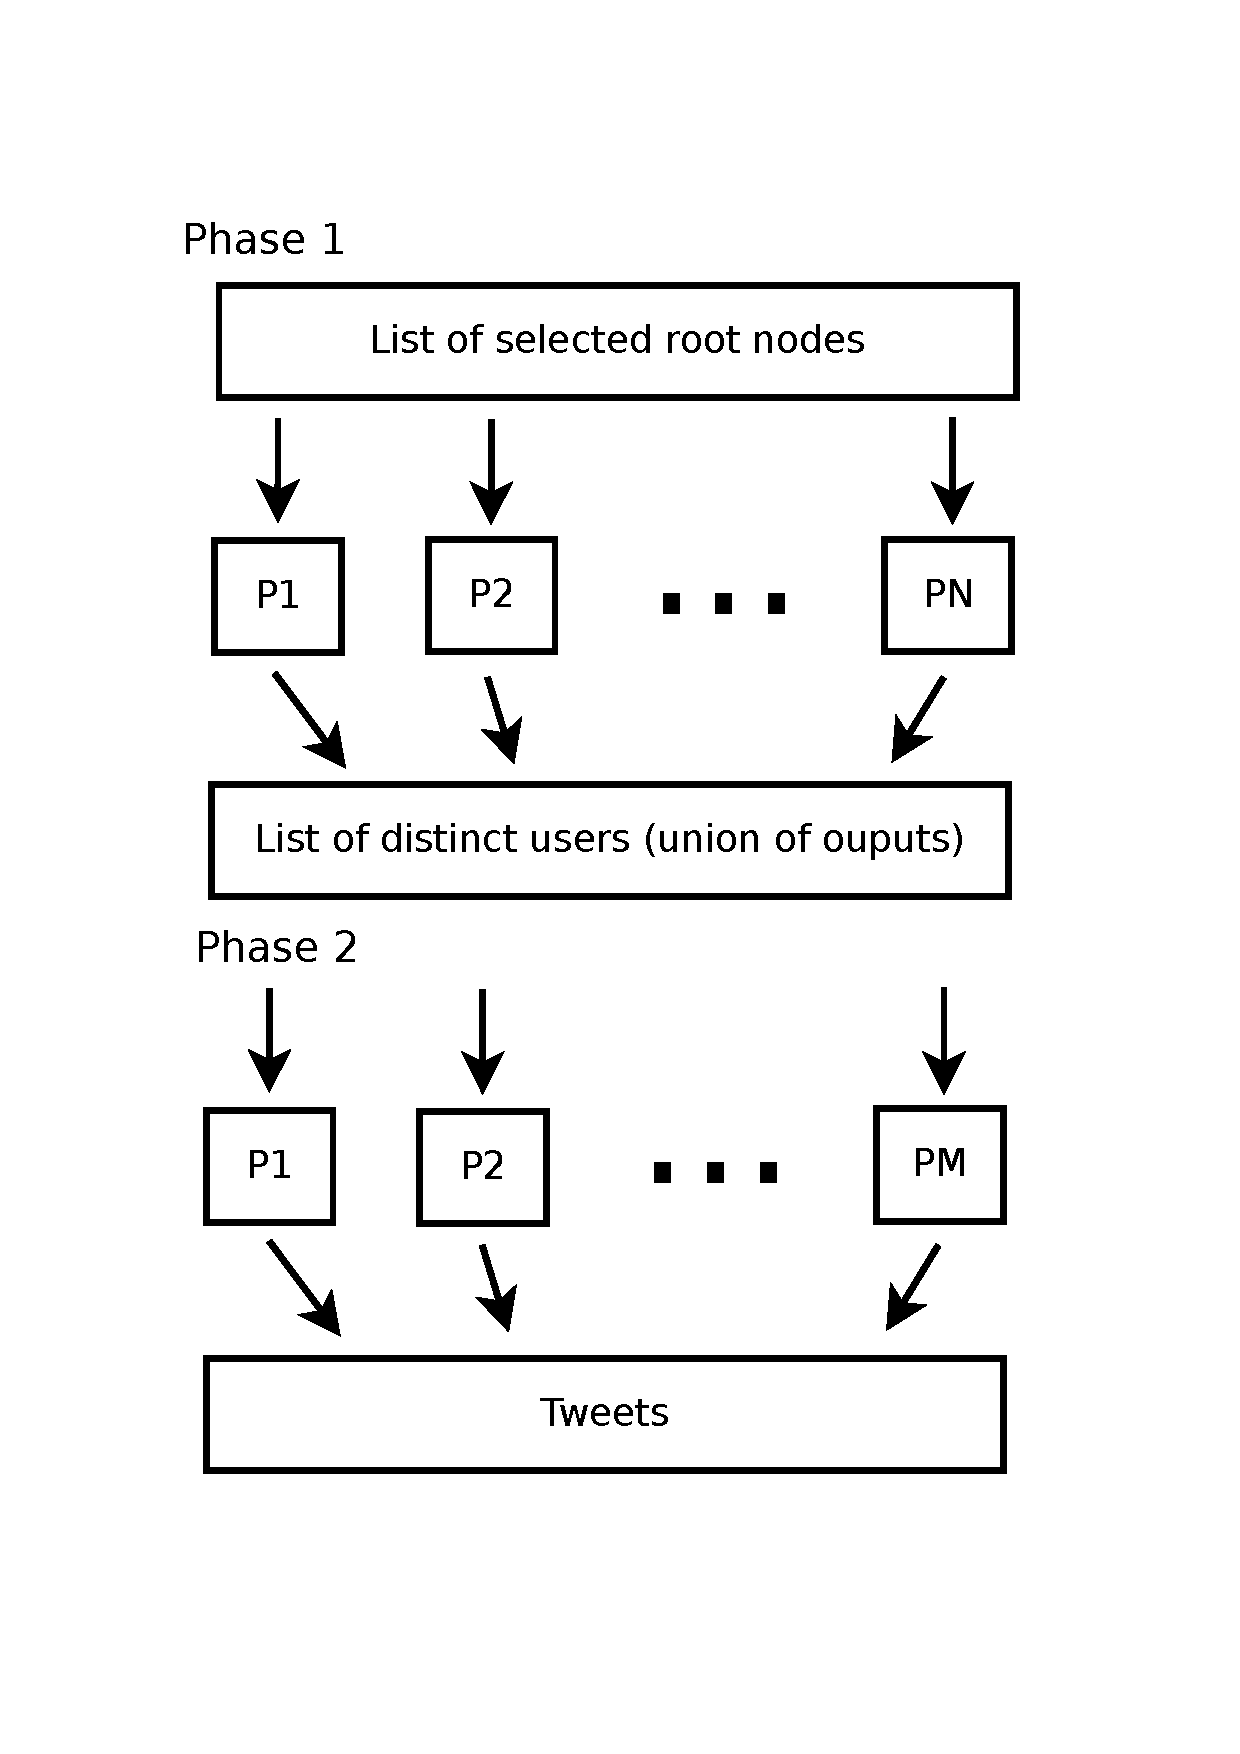
\includegraphics[width=.7\textwidth]{./img/CollectionProcess.pdf}
\caption{Tweet collection methodology.}
\label{fig:methodology}
\end{figure}

\subsubsection*{Approach 2: Filtering tweets provided by webarchive.org}
https://archive.org/details/twitterstream

\subsection*{Daily? tweet aggregator}

\subsubsection*{Clustering according to keywords}

\subsection*{Issue of localization}

\subsubsection*{Geolocalized tweets}
Filtering the available archives of tweets taken from the API yielded near to no geolocalized tweets from India matching our set of keywords. This reason is evident, because the twitter API only allows extraction of 1\% of tweets and only 2\% of tweets are actually geolocalized. In effect, getting tweets that match our keywords specific to food commodities is very unlikely. We had more luck with tweets from Indonesia, however as already explained we were unable to attain enough price sequences from Indonesia to actually train a model. Furthermore, the time constraints didn't allow us to get tweets from India and Indonesia in parallel in order to do some "stand-alone" clustering analysis.

\subsubsection*{Approximation: Mapping tweets to user location}


\section*{Processing}

\subsection*{Merging Series}

\subsection*{Crafting indicators from tweets}

\subsubsection*{Sentiment analysis}

Sentiment analysis, or opinion mining, is the concept of using different computer science techniques (mainly machine learning and natural language processing) in order to extract sentiment information and subjective opinions from the data. In our context this may help us to find out how circumstances in relation to commodity prices affect the overall mood in the population. 

From the start we decided that we did not want to build our own sentiment analysis system since the proper implementation, testing and evaluation would require a considerable effort compared with the total project workload. Instead, we are planning to use some of already developed solutions and tune them to our needs. 

Several sentiment analysis frameworks were tested, including:

\begin{itemize}
\item SentiStrength \par (http://sentistrength.wlv.ac.uk/)

\item Stanford CoreNLP \par (http://nlp.stanford.edu/sentiment/code.html) 

\item 'Pattern' library from the University of Antwerp \par (http://www.clips.ua.ac.be/pages/pattern-en)
\end{itemize}

All of these software packages produced reasonable results on some short and simple sentences, but sentiment grades looked almost random on a set of real collected tweets. Most likely, factors such as misspelled words, acronyms, usage of slang and irony contributed to the overall ambiguity of sentiment grades assignment.

Therefore, we decided to build and use our own simple system, which incorporated basic natural language processing and opinion mining techniques, but was mainly focused on extracting relevant keywords, which could help to estimate tweets from the specific point of view. This approach, which also takes into account issues originating from word misspelling, is described in next two paragraphs.

\subsubsection*{Extracting predictor categories}

First, several "predictor categories" were selected. These categories represent different aspects of price variation, and each category include several sets of words of different polarities. For example, the category "price" has two polarities: "high" and "low". The following word list belongs to "high" polarity: 'high', 'expensive', 'costly', 'pricey', 'overpriced', and these are words from "low" list: 'low', 'low-cost', 'cheap', 'low-budget', 'dirt-cheap', 'bargain'. Likewise, a category "supply" has "high" polarity (with words 'available', 'full', 'enough', 'sustain', 'access', 'convenient') and "low" ('run-out', 'empty', 'depleted', 'rotting'). The dictionary with total of 6 categories (each having at least two polarity word lists) was built ("predict", "price", "sentiment", "poverty", "needs", "supply"), let's call it $D$.

Then, for each tweet a feature vector is built, representing the amount of words from each category and polarity. Several cases have to be taken into account. First of all, a word may be not in its base form ("price" -> "prices", "increase" -> "increasing"), which will prevent an incoming word from matching one from $D$. Therefore, we use stemming technique to reduce each word to its stem (or root) form. Another problem is misspelled words ("increase" -> "incrase", "incraese"), and for tweets it happens more than usual due to widespread use of mobile devices with tiny keyboards. Our solution to this problem is covered in the next section.

Here is the overview of predictor category extraction algorithms we implemented:\\

\textbf{Preprocessing}: For each relevant word in $D$ a stem is computed using the Lancaster stemming method, and the stem is added to reverse index $RI$, which maps a stem to a tuple: (category, polarity). \\

\textbf{function get\_category(w):} 

\indent
\begin{algorithm}[H]
Compute a stem $s$ from $w$ \par
Check if $s$ is present in $RI$. 

  \eIf{yes}{
	\textbf{return} the corresponding tuple.
   }{
		ask spell checker for a suggestion \par
		is suggestion stem returned? \par
		\eIf{yes}{
			\textbf{return} the corresponding tuple from $RI$		
		}{
			\textbf{return} None;
		}
  	}
% \caption{Algo}
\end{algorithm}
\noindent \\

On a high level, every tweet is split into words, and then each word (token) is passed through 'get\_category' function. But here's another problem we face using this approach: each relevant word we met may have a negation word (particle) before it, which subverts the meaning: "increases" -> "doesn't increase", "have food" -> "have no food", etc. To deal with this problem, we employed the following method: we added a special 'negation' category with a list of negation words ("not", "haven't", "won't", etc.), and if there is a word with "negative" category before some relative word (to be more precise, within some constant distance from it, say 2), then we change the polarity of relative word's category. For example, if a word is from category "poverty" and has "high" polarity (like "starving"), then negative category word right before it (such as "aren't") will turn the polarity to "low".


\subsubsection*{Tweets spell checking}

People often do not pay much attention about the proper word spelling while communicating over the Internet and using social networks, but misspelled words may introduce mistakes in processing pipeline and significantly reduce the amount of filtered tweets, since the relevant, but incorrectly written word might not be recognized by the algorithm.

Several spell checking libraries were checked (Aspell and Enchant to name a few), but their 'suggest' method lacked both performance (several seconds to generate a suggestion for thousands words, which is very slow) and flexibility (it's not possible to specify the number of generated suggestions, as well as a threshold, such as maximal edit distance between words). Therefore, we decided to use simple approach which involved computing edit distances between a given word and words from predictor categories dictionary ($D$).

For each given word $w$ we compute its stem $s$ and then edit distance (also known as Levenshtein distance) to each word (stem) from $D$. It can be done really fast thanks to C extensions of \textit{python-levenshtein} module.

After that, we choose the stem with minimal edit distance (using heap to store the correspondence between distances and words and to speed up selection of the minimal one), and check if the resulting number of "errors" (which is equal to distance) is excusable for the length of word $w$. For example, we don't allow errors for words of length 5 or less, only one error is allowed for lengths from 6 to 8, etc. If everything is alright, then the suggestion is returned, otherwise the word is discarded.
 
The approach proved to be fast and tweakable, and was successfully used for tweets processing.
